\section{AFC Frequency Netting}
\label{sec:afc}

The receiver measures the peer's carrier offset on every decoded frame
anyway (\texttt{stats.cfo\_hz}), so the link closes the loop: the
5-bit LC field carries ``shift your carrier by $-X$\,Hz'' requests
($\pm 120$\,Hz per frame, 8\,Hz steps, $\pm 12$\,Hz deadband), and the
peer trims its \emph{shared} reference oscillator.  Trimming the
shared reference moves TX and RX together --- which is exactly why
asking the peer to correct beats retuning locally
(Section~\ref{sec:rf}).  Corrections are applied at \textbf{half
gain}: both sides act on measurements that are one frame stale, and
full-gain corrections would swap the offset between the stations each
turn instead of converging (Figure~\ref{fig:afc}).

\begin{figure}[H]
    \centering
    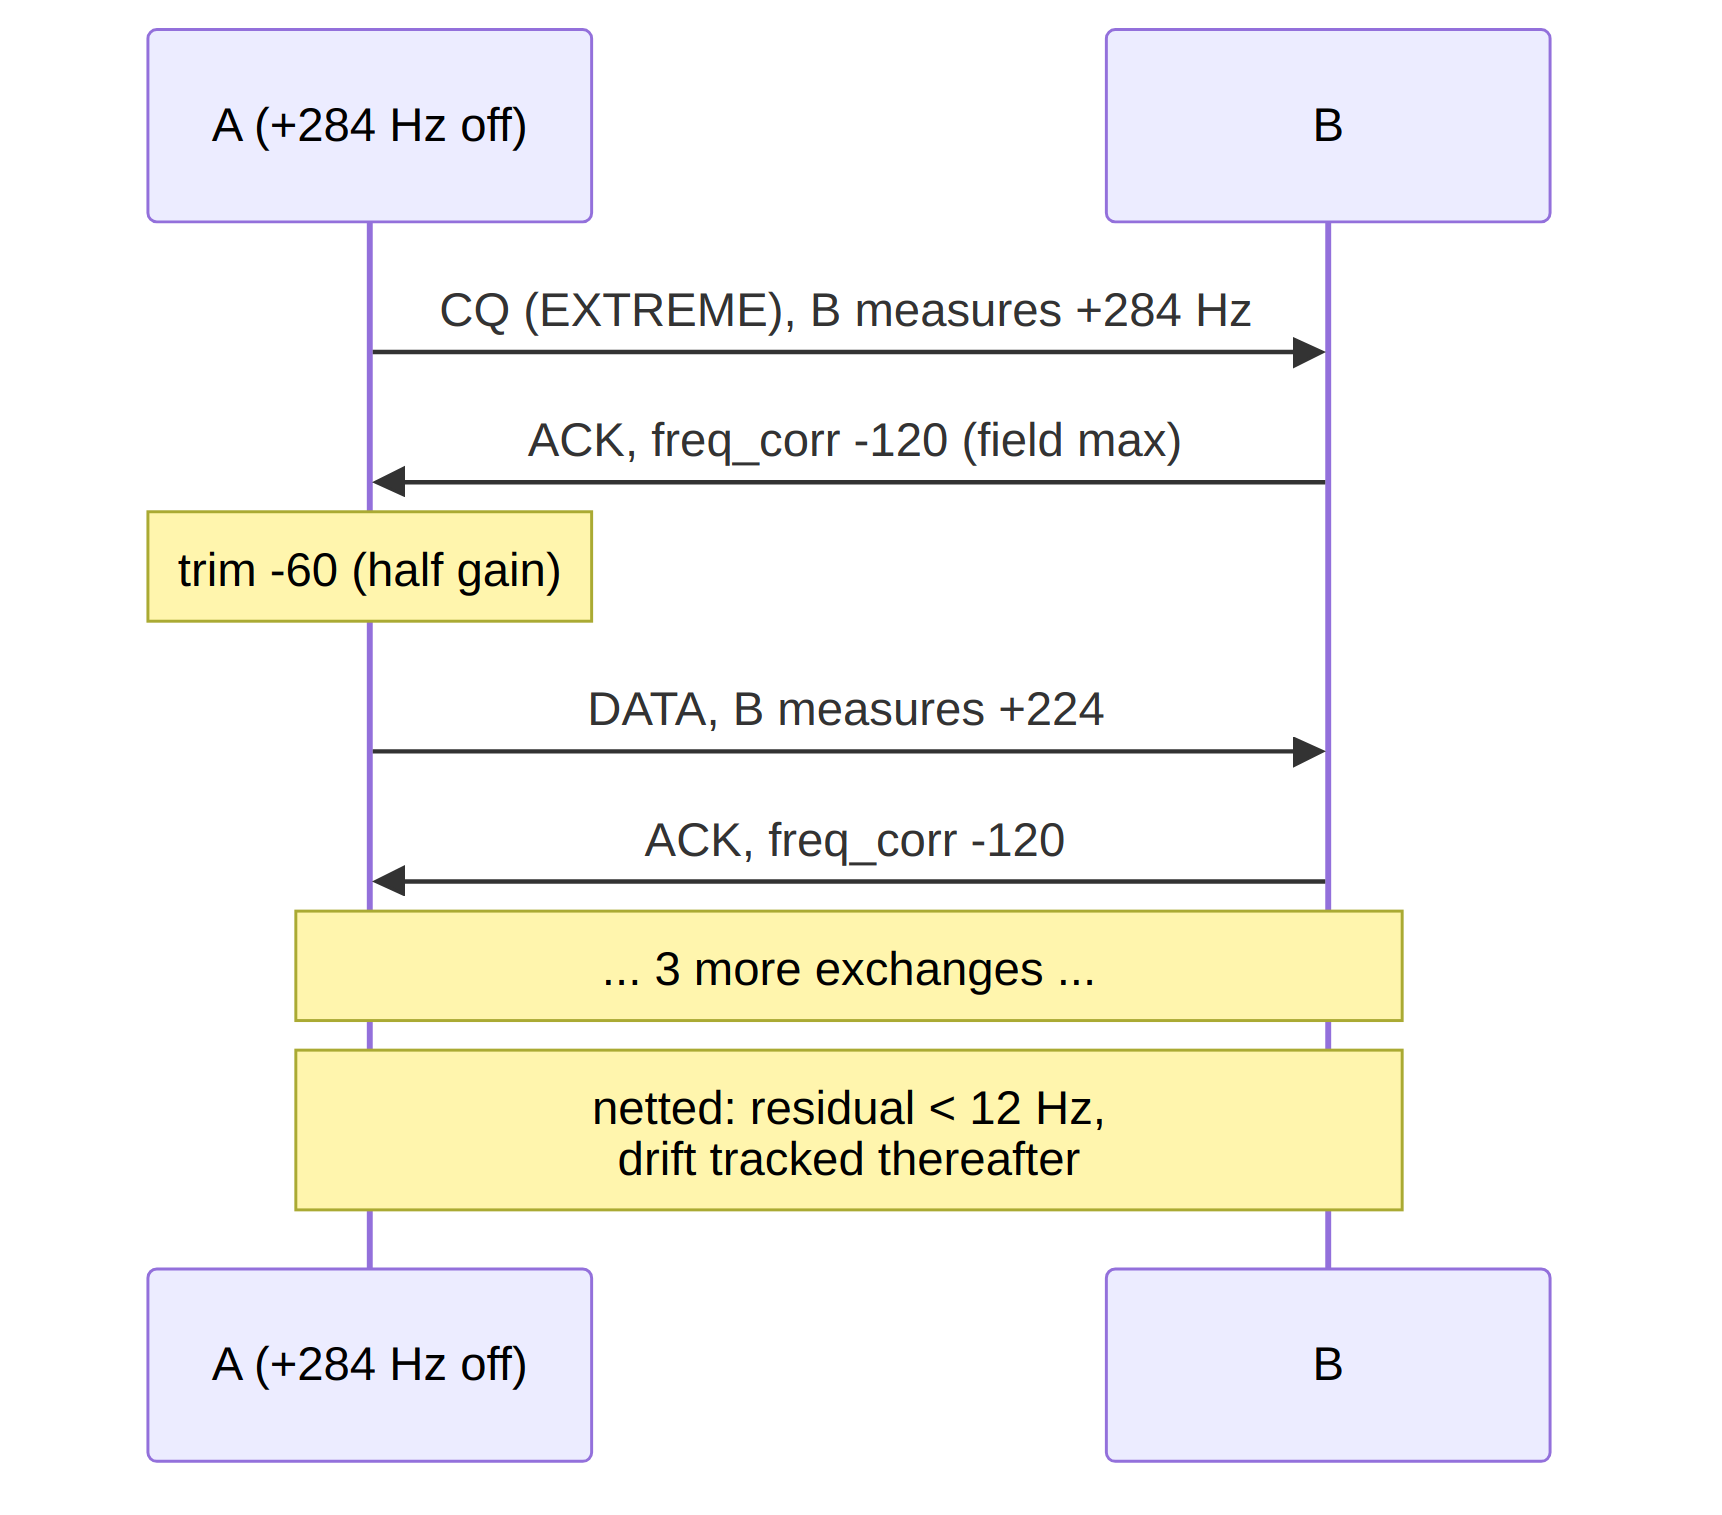
\includegraphics[width=0.85\textwidth]{images/afc_seq.png}
    \caption{AFC netting from a $+284$\,Hz initial offset.}
    \label{fig:afc}
\end{figure}

\subsection{Guard Rails}

The loop observes only the \emph{differential} offset, so without
bounds the pair's common frequency random-walks over a long session
--- out of the channel slot, into bystanders' passbands, or off the
rig's trim range.  Two mechanisms bound it:

\begin{itemize}
    \item \texttt{afc\_max\_trim\_hz} (default $\pm 150$\,Hz)
          hard-clamps each station's \emph{cumulative} trim.  Requests
          beyond the budget are partially honoured or refused, the
          peer's own headroom carries the rest, and any residual is
          left to the modem's $\pm 300$\,Hz CFO tolerance --- the link
          keeps working, just without full netting.
    \item \texttt{afc\_anchor=True} designates a station (e.g.\ the CQ
          caller) that never trims, pinning the absolute frequency
          entirely; the peer does all the correcting.
\end{itemize}

\subsection{Measured Behaviour}

\texttt{experiments/afc\_netting.py} runs two worn-TCXO rigs on
14.2\,MHz starting \textbf{$+284$\,Hz apart} (near the modem's
$\pm 375$\,Hz limit) with opposing thermal drifts: netted to within
the deadband in $\approx$5 correction exchanges ($\approx$104\,s ---
EXTREME bootstrap frames dominate the wall clock), steady-state
$|$CFO$| \le 11$\,Hz under continuing 0.09\,Hz/s relative drift,
400/400 bytes delivered.  The guard scenarios behave as designed:
default budgets net fully (final $|$CFO$|$ 3\,Hz, trims clamped at
$-150/+144$\,Hz); deliberately tight $\pm 40$\,Hz budgets stop at
their limits leaving a 222\,Hz residual \emph{by design}, with the
link still delivering on CFO tolerance alone; an anchored station A
forces B to absorb the full $+292$\,Hz and the pair's absolute
frequency never moves.  Beyond robustness margin, a netted link could
shrink EXTREME's per-symbol frequency-search range (compute) and eases
mask-grid detection at the extremes.
